\documentclass[12pt,a4paper,oneside]{report}
\usepackage{fontspec}
\setmainfont{Times New Roman}
\setsansfont{Arial}
\usepackage[top=3.5cm,bottom=3cm,left=3.5cm,right=2cm,headheight=16pt,headsep=1cm]{geometry}
\usepackage{graphicx,array,longtable,booktabs,caption,titlesec,fancyhdr,xurl,hyperref}
\hypersetup{hidelinks,pdftitle={UI Automation Testing in Flutter},pdfauthor={Nguyễn Bá Hùng and Nguyễn Bảo Long}}
\urlstyle{same}
\makeatletter
\renewcommand\normalsize{\@setfontsize\normalsize{13pt}{19.5pt}}
\makeatother
\AtBeginDocument{\normalsize}
\setlength{\parindent}{1.27cm}
\setlength{\parskip}{0pt}
\setlength{\emergencystretch}{2em}
\widowpenalty=10000\clubpenalty=10000
\pagestyle{fancy}\fancyhf{}\fancyhead[C]{\thepage}\renewcommand{\headrulewidth}{0pt}
\fancypagestyle{plain}{\fancyhf{}\fancyhead[C]{\thepage}\renewcommand{\headrulewidth}{0pt}}
\titleformat{\chapter}[hang]{\bfseries\fontsize{16}{20}\selectfont}{\thechapter}{0.7em}{}
\titlespacing*{\chapter}{0pt}{0pt}{16pt}
\titleformat{\section}{\bfseries\fontsize{14}{18}\selectfont}{\thesection}{0.7em}{}
\titlespacing*{\section}{0pt}{12pt}{6pt}
\setcounter{tocdepth}{1}
\captionsetup{font={small,it},labelfont=it,justification=centering}
\begin{document}\hypersetup{pageanchor=false}

\begin{titlepage}\thispagestyle{empty}\centering
{\fontsize{14}{18}\selectfont VIETNAM GENERAL CONFEDERATION OF LABOUR\\\textbf{TON DUC THANG UNIVERSITY}\\\textbf{FACULTY OF INFORMATION TECHNOLOGY}\par}
\vspace{0.7cm}
\includegraphics[width=3.1cm]{assets/tdtu-logo.png}\par\vspace{0.8cm}
{\bfseries\fontsize{14}{19}\selectfont NGUYỄN BÁ HÙNG\\NGUYỄN BẢO LONG\par}\vspace{1cm}
{\bfseries\fontsize{22}{27}\selectfont UI AUTOMATION TESTING\\IN FLUTTER\\IMPLEMENTING END-TO-END TESTING\par}\vspace{0.8cm}
{\bfseries\fontsize{18}{23}\selectfont MIDTERM REPORT\\SOFTWARE ENGINEERING\par}\vspace{0.6cm}

Cross-Platform Mobile App Development — 503107\\Class 23K50201\\Semester 1, Academic Year 2026–2027\par\vfill HO CHI MINH CITY 2026\end{titlepage}

\begin{titlepage}\thispagestyle{empty}\centering
{\fontsize{14}{18}\selectfont VIETNAM GENERAL CONFEDERATION OF LABOUR\\\textbf{TON DUC THANG UNIVERSITY}\\\textbf{FACULTY OF INFORMATION TECHNOLOGY}\par}
\vspace{0.7cm}
\includegraphics[width=3.1cm]{assets/tdtu-logo.png}\par\vspace{0.8cm}
{\bfseries\fontsize{14}{19}\selectfont NGUYỄN BÁ HÙNG — 523K0006\\NGUYỄN BẢO LONG — 523K0014\par}\vspace{1cm}
{\bfseries\fontsize{22}{27}\selectfont UI AUTOMATION TESTING\\IN FLUTTER\\IMPLEMENTING END-TO-END TESTING\par}\vspace{0.8cm}
{\bfseries\fontsize{18}{23}\selectfont MIDTERM REPORT\\SOFTWARE ENGINEERING\par}\vspace{0.6cm}
Instructor: Mai Văn Mạnh\par\vspace{0.35cm}
Cross-Platform Mobile App Development — 503107\\Class 23K50201\\Semester 1, Academic Year 2026–2027\par\vfill HO CHI MINH CITY 2026\end{titlepage}

\pagenumbering{roman}\hypersetup{pageanchor=true}\chapter*{ABSTRACT}
This report investigates UI automation testing through TaskFlow, a Flutter task-management application with isolated offline, sample and account workspaces. The study connects unit, widget, golden, native integration and browser tests to specific risks rather than treating test count as a quality measure. Injectable repositories, clocks and identifiers support deterministic fixtures, while explicit completion gates expose loading and recovery states. The account implementation adds a Node.js and SQLite boundary with ownership checks and revision-based snapshot writes. A deliberate substring-to-prefix search defect is detected by a permanent regression, with authentic baseline, failure and corrected outputs. Three rounds of selected test-level commands illustrate local wall-time differences, but unequal workloads and startup overhead prevent a universal speed ranking. During report preparation, the updated Flutter suite passed 100 cases and the backend suite passed 14 cases. Retained Windows and Edge evidence and historical Android CI results are reported with their revision and platform boundaries. These selected checks do not establish absence of defects or unconditional release readiness. The study concludes that clear oracles, isolated state, complementary execution boundaries and honest interpretation are central to a defensible Flutter testing case study.


\noindent\textit{Keywords: Flutter; UI automation; integration testing; regression; reproducibility.}
\tableofcontents\clearpage\listoffigures\listoftables\clearpage\pagenumbering{arabic}
\chapter{Introduction}
\section{Problem and motivation}
Task management becomes difficult when an application must preserve records, validate metadata, recover from failed writes and remain usable across screen sizes. A successful tap does not prove that a task was saved; a correct screenshot does not prove that search returns the right records. These differences motivate testing at several boundaries rather than treating one framework as a complete quality strategy.

This report addresses Topic 4, UI Automation Testing in Flutter: Implementing End-to-End Testing, for Cross-Platform Mobile App Development, course 503107. The demonstration application is TaskFlow, a Flutter task manager developed as a testing case study. Its offline mode uses local preferences, its sample mode is temporary, and its account mode communicates with a Node.js and SQLite backend. The backend is included because it exposes realistic failure and concurrency conditions, not because the report attempts to become a general backend-development survey.

The September 2026 desktop refactor illustrates this problem: widget and golden checks passed after intentional visual updates, while Edge automation still required correction because its readiness and focused-input assumptions described the previous interface.

\section{Objectives and research questions}
The objectives are to explain deterministic Flutter testing mechanisms, apply them to meaningful workflows and interpret the resulting evidence. The explanation covers finders, frame scheduling, dependency injection and the distinction between controlled fakes and real persistence.

Four questions organize the study. RQ1 asks which risks are best addressed by unit, widget, golden, native integration and browser tests in this application. RQ2 asks whether a meaningful automated workflow can detect a deliberate semantic defect that does not prevent compilation. RQ3 asks how isolation, explicit completion gates and observable-state assertions affect reproducibility. RQ4 asks what can legitimately be concluded from local test results, limited repetition experiments and historical hosted Android evidence.

The contribution is an inspectable case study, not a new testing algorithm. It connects implementation decisions to tests for persistence, drafts, account isolation and visual change control.

\section{Scope and evaluation boundary}
The application supports creating, editing, completing, searching, filtering, sorting and deleting tasks. Records contain a title, optional notes, priority, due date and normalized tags. Deletion has a one-level undo during the current session. Account workflows cover registration, sign-in, profile changes, recovery codes, password changes, session revocation and account deletion. Offline data is not silently uploaded when a user signs in.

Implementation claims describe inspected code; measured claims describe retained runs. Proposed improvements and missing evidence are labelled separately. A runnable backend, for example, does not establish production readiness or sustained-load capacity.

The evaluated source is baseline commit 39dd199 on branch main-test plus the verified draft-consistency update in the working tree. The review reran the Flutter and backend suites and a Windows draft-exit workflow. Historical Windows, Edge and Android results retain their original dates and revisions. This manuscript describes the corrected implementation and completed experiments within their stated verification boundaries.

\section{Research and evidence method}
The technical explanation combines official framework documentation with a source-level examination of TaskFlow. Documentation establishes API behavior; project code establishes how that behavior is used here. Tests establish only the observations asserted under their recorded conditions. The study therefore avoids inferring a real Android run from a golden test configured with an Android rendering variant, or inferring an operating-system restart from a widget remount.

Evidence was collected through deterministic fixtures, standard runner output, controlled failure injection and separate platform invocations. The intentional search experiment preserves baseline, failing and corrected outputs. The timing experiment reports whole-command durations for unequal selected suites and explicitly includes native compilation and launch overhead. Browser results preserve unsuccessful attempts instead of replacing them with the final successful rerun.

\section{Report organization}
Chapter 2 explains the test mechanisms and compares the approaches used in the project. Chapter 3 translates product requirements into risks and observable acceptance conditions. Chapter 4 describes the architecture, data model and security boundaries. Chapter 5 connects those designs to implementation and platform behavior. Chapter 6 presents the test design, experimental results, audit findings and threats to validity. Chapter 7 concludes with the supported findings and prioritized remaining work. The appendices provide a compact reproduction guide and an evidence index rather than reproducing long raw logs.

\chapter{Testing foundations and comparative analysis}
\section{Different tests answer different questions}
Flutter distinguishes unit tests, widget tests and integration tests by the boundary under examination. Its testing overview recommends combining many focused tests with sufficient integration coverage of important use cases, while recognizing differences in dependencies, speed and maintenance (Flutter, n.d.-a). TaskFlow adds golden comparisons as a visual oracle and browser automation as an external check of the Web interface. These mechanisms overlap in coverage but are not interchangeable.

A unit test of TaskFilters can construct records directly and check the exact output order. It does not need a rendered search box or a device. A widget test can type a query into TaskScreen and check the resulting task widgets. This verifies the connection between an input event, controller filtering and the displayed list, while still allowing a fake repository. A native integration workflow uses an actual Windows application process and, in the persistence suites, the preference plugin. Its additional value is crossing those platform and storage boundaries, not merely executing a longer sequence of taps.

Figure 2.1 summarizes the evidence layers used in TaskFlow. The shape is a design principle rather than a measured ratio: inexpensive, focused checks should localize most rule failures, while selected workflows cover interactions that lower layers cannot establish. Golden and browser tests complement this structure rather than replacing its foundation.

\begin{figure}[htbp]\centering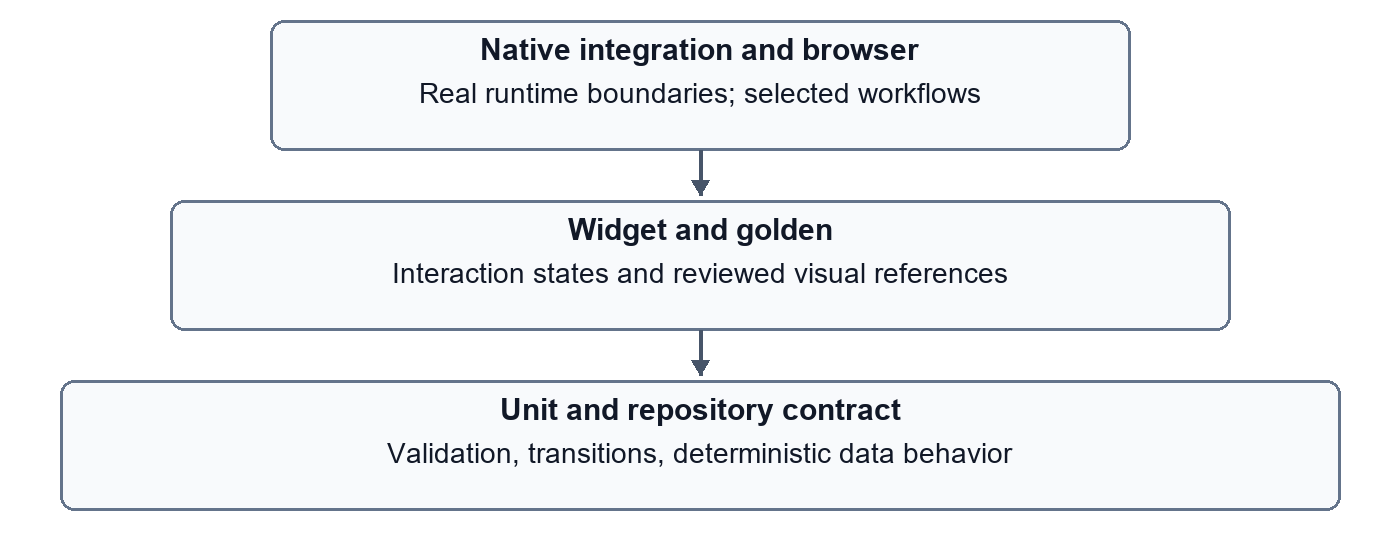
\includegraphics[width=\linewidth]{assets/testing-layers.png}\caption{Testing layers and their TaskFlow evidence boundaries}\end{figure}
\section{Binding and frame scheduling}
A Flutter widget test requires a binding that coordinates the framework, rendered tree and test actions. The fixture mounts the app with pumpWidget, supplies dependencies and advances frames deliberately. The official pump API documents an important distinction: advancing time in a fake-async test environment differs from delaying a live test for the same duration (Flutter, n.d.-b). Therefore, a duration used in a widget fixture must not automatically be interpreted as a user-perceived delay on a device.

In TaskFlow, an asynchronous repository operation changes controller state before it produces a result. The controller sets busy, clears an earlier error and notifies listeners. The screen can now display loading and disable mutation actions while the repository future remains incomplete. When the future completes, the controller publishes either the confirmed task list or an error. A test that asserts only the final list can miss a broken intermediate state, such as an Add button remaining active and allowing duplicate work.

The loading tests use a Completer to keep the operation pending. They pump the initial frame, inspect the loading state, release the gate and only then settle the interface. This makes the relevant state observable without assuming a particular processor speed. A fixed sleep would instead mix the repository contract with host scheduling: it might be unnecessarily slow on one machine and too short on another.

\section{Settling and bounded waiting}
pumpAndSettle repeatedly pumps frames until no frame remains scheduled, with a timeout. Its documentation warns that an indeterminate animation can prevent settling and recommends understanding the number of frames required by the interaction (Flutter, n.d.-c). TaskFlow has exactly this risk while an unresolved repository gate keeps a progress indicator active. Calling settle before completing the gate would wait for a condition that the test itself prevents.

The practical rule is to choose the wait from the expected state transition. During a controlled pending operation, pump enough to observe the frame and assert the disabled action. After completing a deterministic gate, settle the resulting short transition. In an external browser, wait for a visible message, task or verified focused input. During native application startup, retain build and connection logs because a timeout may occur before any business assertion runs.

The project also demonstrates the limitation of a timeout value. An earlier combined native invocation could not establish the next debug connection, while a separate unchanged invocation passed. Other retained native runs stalled during a workflow and required a standalone rerun. These observations do not identify a root cause. Increasing the timeout until a test passes would obscure whether the problem is application behavior, driver connectivity or the host environment.

\section{Finders and meaningful assertions}
Finders connect a test action to a specific target. A key is useful when several controls have similar text, while a visible label helps express user intent. Flutter's byKey finder skips offstage widgets by default, which matters for hidden detail forms and inactive routes (Flutter, n.d.-d). A test that deliberately includes offstage elements needs a reason; otherwise it may interact with content the user cannot currently reach.

TaskFlow uses stable keys for metadata fields and visible text for actions such as Add task, Save changes and Retry. Task assertions are scoped to CheckboxListTile rather than the entire tree. Without that scope, a search test could succeed because the query text remained in the input field even though the expected task had disappeared. The permanent substring-search regression test checks the task row itself and also excludes an unrelated record.

Exact order is another important oracle. Checking that Alpha and Beta are both present does not establish that sorting works. The discovery scenarios compare the ordered result set after normalized search, status, priority and tag constraints have been combined. They also restore the unfiltered order through Clear filters, so a partially reset filter cannot pass by leaving an apparently plausible list.

\section{Fakes and dependency injection}
The TaskRepository interface separates application behavior from storage. The in-memory implementation can delay or fail operations, the local implementation uses preferences, and the remote implementation exchanges revisioned snapshots with the API. Clock and ID generation are injectable in TaskController. A fixture can therefore define both temporal boundaries and stable identities instead of inheriting the machine's current date or generating unpredictable task keys.

A fake is a simplified working implementation, not a guarantee that the real dependency behaves identically. The in-memory repository is appropriate for inspecting error states because the failure can be produced at a known point. It cannot establish serialization compatibility with the preference plugin or isolation between two API accounts. Those questions require separate tests at the actual boundary. The project intentionally retains both controlled-repository scenarios and real-preference scenarios for this reason.

Test independence requires more than constructing a new screen. A repository object, storage key, unresolved future, test-input registration or viewport override can survive into another test if cleanup is incomplete. The native suites use dedicated preference keys and bounded helpers, and register and unregister the test text-input channel. They do not clear all preferences, which would risk deleting unrelated user data and weaken the precision of the test environment.

\section{Golden tests and visual change control}
The matchesGoldenFile matcher compares rendered output against an expected image. The API supports images obtained from a finder, image object or bytes; finding the correct rendering boundary is part of fixture design (Flutter, n.d.-e). TaskFlow compares selected screens with fixed dimensions, vendored font fixtures and a controlled target-platform variant. The comparator supplies a visual difference signal, not an explanation of whether the new image is desirable.

The minimalist UI update changed background, accent, branding, capture layout and workspace navigation. Fifteen reference images were therefore intentionally reviewed and replaced. Treating every pixel difference as a defect would block a requested redesign. Automatically accepting every new image would remove the regression oracle. The required middle step is visual review: confirm that the difference corresponds to the intended change and that text, dialogs and actions remain readable.

Goldens are not sufficient accessibility evidence. A screenshot may look correct while a control has an empty accessible label. Conversely, a correctly labelled control may overflow at enlarged text. TaskFlow combines semantics checks, layout tests and visual baselines, and keeps manual screen-reader verification as a separate outstanding activity.

\section{Native integration and browser automation}
The integration\_test package lets an application-level workflow use Flutter testing APIs while running on a supported target. The official guide describes desktop, device and browser workflows, including driver-based browser setup (Flutter, n.d.-f). The local SDK rejected the specific direct Edge invocation attempted in this project. That recorded limitation must not be generalized into a claim that Flutter has no browser integration-testing route.

TaskFlow uses a compile-time-gated Web harness for deterministic browser validation, discovery and retry scenarios. It contains synthetic in-memory data and no API client. Playwright locators can use roles and accessible names and resolve their targets again for subsequent actions; its documentation also notes that role locators are not a substitute for an accessibility audit (Microsoft, n.d.). The actual-browser check complements widget testing because it observes Flutter's generated DOM semantics and browser focus behavior.

Patrol is a relevant alternative when test workflows need additional native interaction. Its documentation introduces a CLI, package integration and native setup requirements (LeanCode, n.d.). Patrol was reviewed as an alternative, not installed or benchmarked in this project. Adding another framework without a corresponding uncovered risk would increase setup and maintenance while contributing little new evidence to the current task-management scenarios.

Table 2.1 expresses the project's decision criteria. The entries are a qualitative assessment of the implemented fixtures, not measured universal rankings of frameworks.

{\fontsize{11}{14}\selectfont\setlength{\tabcolsep}{4pt}\renewcommand{\arraystretch}{1.15}
\begin{longtable}{@{}>{\raggedright\arraybackslash}p{0.21\linewidth}>{\raggedright\arraybackslash}p{0.34\linewidth}>{\raggedright\arraybackslash}p{\dimexpr0.45\linewidth-16pt\relax}@{}}
\caption{Test selection for TaskFlow risks}\\\toprule
\textbf{APPROACH} & \textbf{STRONGEST LOCAL USE} & \textbf{IMPORTANT LIMIT} \\ \midrule
\endfirsthead\toprule
\textbf{APPROACH} & \textbf{STRONGEST LOCAL USE} & \textbf{IMPORTANT LIMIT} \\ \midrule
\endhead
Unit & Validation and deterministic transformations & No rendered interaction \\ \addlinespace[5pt]
Widget & Form states, actions and draft preservation & Controlled environment and storage \\ \addlinespace[5pt]
Golden & Reviewed visual states at fixed sizes & Font and rendering sensitivity \\ \addlinespace[5pt]
Native integration & Plugin persistence and complete workflows & Build and driver complexity \\ \addlinespace[5pt]
Browser harness & DOM semantics and browser interaction & Synthetic repository in this harness \\ \addlinespace[5pt]
Node API tests & Authentication, isolation and revisions & No Flutter rendering \\ \addlinespace[5pt]
\bottomrule\end{longtable}}
\chapter{Requirements and risk analysis}
\section{Actors and workspace modes}
TaskFlow has three user-facing workspace modes. An offline user manages tasks stored on the current device. A sample user explores temporary seeded tasks that are discarded on exit. An account user manages server-backed records belonging to the authenticated account. These modes share the task interface but differ in persistence, recovery and privacy boundaries. There is no background transfer from offline storage to the account backend.

The sample mode is an important part of reproducible demonstration. A presenter can search, edit and delete synthetic tasks without changing saved coursework data or creating a server account. Re-entering the sample recreates its known state. The interface must communicate that this is a session-only workspace; presenting it as synchronized or permanently saved would be a UX defect even if every button worked correctly.

The backend actor is the authenticated account, not an arbitrary user identifier supplied in a task request. Ownership is derived from the session. A request that knows another account's task ID must still be unable to read or change that account's record. This requirement is tested separately from the visible task-management flow because it is fundamentally an authorization property.

\section{Functional requirements and acceptance conditions}
A valid task title is required and is normalized before persistence. Optional details include notes, a priority chosen from low, medium and high, a calendar date and normalized tags. Creation must produce exactly one stored record with stable identity; editing must preserve identity and creation time. Marking completion changes the task state without discarding its other fields. Deletion asks for confirmation, and undo restores the most recent deleted record during the current session.

Search normalizes surrounding whitespace and case. It examines title, notes and tags, while the exact-tag filter compares normalized tag values. Status, priority, due-date and tag filters combine rather than replace each other. Sorting must be deterministic, including ties. Clearing filters must reset both the visible query and filter state. Table 3.1 links these requirements to observable checks rather than to the presence of a screen or source file.

{\fontsize{11}{14}\selectfont\setlength{\tabcolsep}{4pt}\renewcommand{\arraystretch}{1.15}
\begin{longtable}{@{}>{\raggedright\arraybackslash}p{0.21\linewidth}>{\raggedright\arraybackslash}p{0.34\linewidth}>{\raggedright\arraybackslash}p{\dimexpr0.45\linewidth-16pt\relax}@{}}
\caption{Functional acceptance matrix}\\\toprule
\textbf{FEATURE} & \textbf{OBSERVABLE ACCEPTANCE CONDITION} & \textbf{MAIN EVIDENCE} \\ \midrule
\endfirsthead\toprule
\textbf{FEATURE} & \textbf{OBSERVABLE ACCEPTANCE CONDITION} & \textbf{MAIN EVIDENCE} \\ \midrule
\endhead
Create & One valid record appears and survives remount & Persisted create scenario \\ \addlinespace[5pt]
Validate & Readable error and corrected successful save & Widget and native validation \\ \addlinespace[5pt]
Discover & Exact matching set and deterministic order & Independent discovery scenario \\ \addlinespace[5pt]
Edit and complete & Updated fields and unaffected metadata survive & Persisted edit scenario \\ \addlinespace[5pt]
Delete and undo & Confirmation and full-record restoration & Native workflow \\ \addlinespace[5pt]
Recover & Failure is visible and retry retains relevant draft & Controlled repository tests \\ \addlinespace[5pt]
Isolate accounts & One account cannot access another's tasks & API and online workflow \\ \addlinespace[5pt]
Preserve visual usability & Compact, wide and enlarged text remain usable & Layout and golden tests \\ \addlinespace[5pt]
\bottomrule\end{longtable}}
\section{Nonfunctional requirements}
Responsiveness is represented by observable intermediate states, not by an unmeasured performance claim. Repository work must not make the interface silently appear successful. The screen displays loading, disables duplicate mutations and offers a clear recovery action after failure. Selected loading tests validate their asserted scenarios, not every possible asynchronous interaction.

Accessibility requirements include readable labels, semantic headings, usable targets, keyboard interaction and layouts that tolerate enlarged text. The desktop search shortcut must actually focus the input. Status and priority must have text meaning rather than color alone. Automated checks can detect several violations, but a passing guideline test does not establish complete WCAG conformance or successful use with a particular screen reader.

Reproducibility requires a known initial state, retained dependency lockfile, documented platform configuration, synthetic test data and evidence that can be mapped to a command and environment. A generated Android folder is insufficient platform evidence. A release executable without its required neighboring Windows files is also insufficient distribution evidence. These requirements shape the documentation and artifact strategy as much as the application code.

\section{Risk priorities}
The highest data-integrity risks are overwriting an unknown snapshot, replaying an uncertain remote save, crossing account boundaries and discarding a user's unsaved changes. Visual polish has value, but it does not compensate for these failures. A second priority is interaction ambiguity: duplicate submissions, hidden validation, unreachable controls, inaccessible labels and unclear workspace persistence. A third is evidence ambiguity, such as attributing a historical CI result to newer source or confusing remount with process restart.

Table 3.2 records the risk-oriented reasoning behind the test design. Severity here is a project triage judgment, not a formal security certification. It guides the order of further investigation and does not imply that all possible risks have been enumerated.

{\fontsize{11}{14}\selectfont\setlength{\tabcolsep}{4pt}\renewcommand{\arraystretch}{1.15}
\begin{longtable}{@{}>{\raggedright\arraybackslash}p{0.21\linewidth}>{\raggedright\arraybackslash}p{0.34\linewidth}>{\raggedright\arraybackslash}p{\dimexpr0.45\linewidth-16pt\relax}@{}}
\caption{Risk controls and remaining evidence gaps}\\\toprule
\textbf{RISK} & \textbf{IMPLEMENTED CONTROL} & \textbf{REMAINING BOUNDARY} \\ \midrule
\endfirsthead\toprule
\textbf{RISK} & \textbf{IMPLEMENTED CONTROL} & \textbf{REMAINING BOUNDARY} \\ \midrule
\endhead
Unknown local snapshot overwritten & Successful load required before mutation & External storage corruption recovery \\ \addlinespace[5pt]
Timed-out remote save replayed & Revision invalidated until reload & Manual conflict resolution \\ \addlinespace[5pt]
Cross-account record access & Session-derived owner and scoped SQL & Independent security assessment \\ \addlinespace[5pt]
Accidental workspace exit & Explicit draft-discard confirmation & OS close and browser reload \\ \addlinespace[5pt]
Visual regression & Reviewed goldens and large-text tests & Full manual assistive-technology use \\ \addlinespace[5pt]
Misleading platform claim & Dated platform evidence with exact scope & Clean-device release installation \\ \addlinespace[5pt]
\bottomrule\end{longtable}}
\section{Investigation boundaries}
The project deliberately excludes collaboration, chat, real-time synchronization, social features and automated offline migration. The backend is a local development service with account functionality; there is no claimed SMTP service, email verification or multi-factor authentication. The report also does not equate a memory-only token policy with complete endpoint or operating-system security.

This bounded scope is suitable for the selected testing topic because it provides enough interactions to expose realistic defects without requiring unrelated infrastructure. The acceptance criterion is explanatory and reproducible evidence about those interactions. Adding a new feature is justified only when it addresses a specific requirement or uncovers a testing mechanism that the existing demonstration cannot show.

\chapter{System design}
\section{Architecture and dependency direction}
TaskFlow separates presentation, application decisions and storage. The task screen renders controller state and collects user intent. TaskController coordinates validation, mutation and error reporting. TaskRepository defines the load and save boundary. Local preferences, the controlled in-memory repository and the HTTP repository satisfy the same contract. Domain records do not need to know whether a task was loaded from a browser preference store or a remote SQLite database.

This arrangement makes the test boundary explicit. A widget test can mount the real task screen and controller with a controllable repository. A persistence test can replace that repository with the real preferences implementation while retaining the same user workflow. An account integration test additionally exercises the client, HTTP transport and database. The interface reduces duplicated interaction code, but it does not make those environments equivalent: only the latter tests cross the corresponding production boundaries.

\begin{figure}[htbp]\centering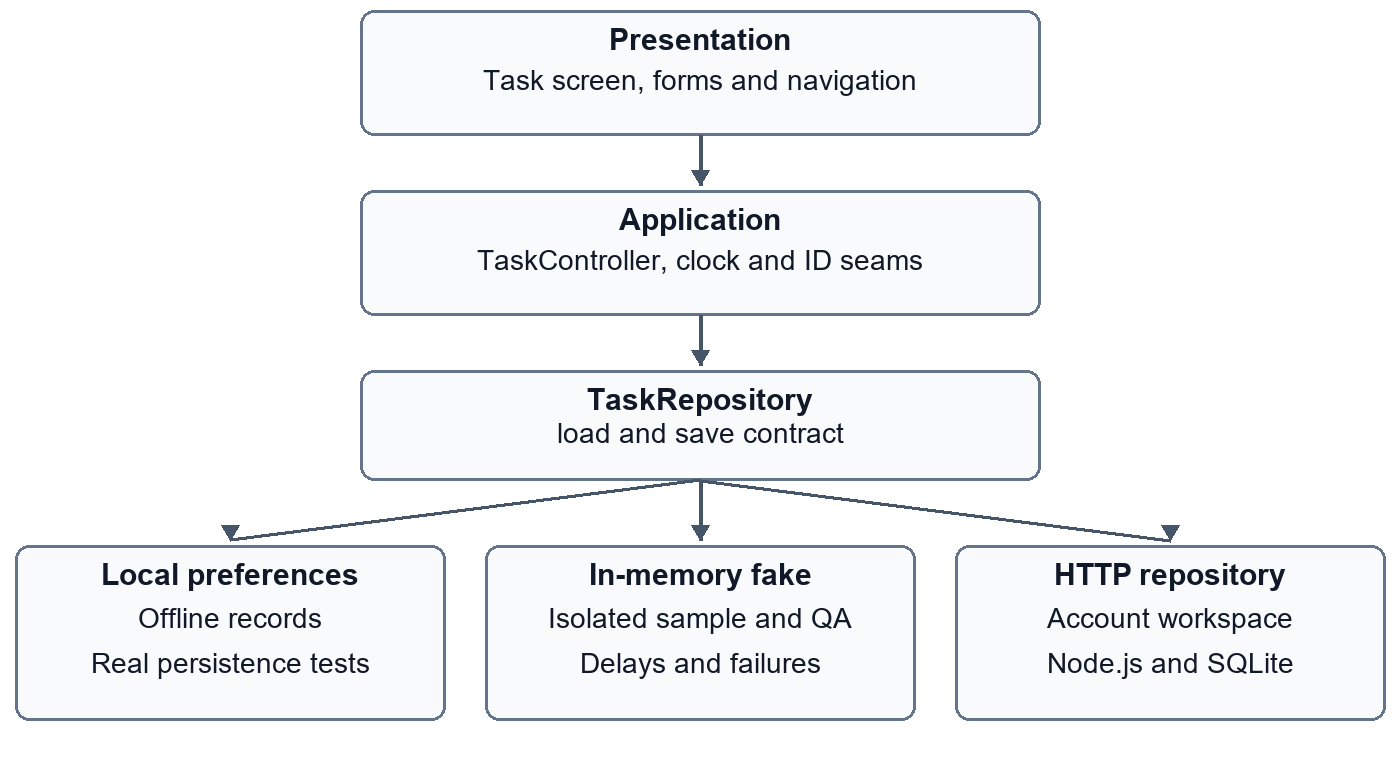
\includegraphics[width=\linewidth]{assets/architecture.png}\caption{Dependency boundaries and the three repository modes}\end{figure}
The controller receives a clock and an identifier generator. Tests can therefore expect a particular record identity and creation time instead of depending on the wall clock or an unpredictable identifier. This is especially important for deterministic ordering and for checking that editing preserves identity. It also prevents an apparently successful edit from being mistaken for deletion followed by creation of a different record.

The account feature introduces a separate session lifecycle. Authentication gates entry to the remote workspace, while the offline and sample entries remain available independently. A sign-in does not migrate local records. That explicit separation avoids an ambiguous ownership decision and makes account-isolation tests meaningful: a task in one workspace must not appear merely because the same device previously opened another workspace.

\section{Domain model and persistence representation}
A task contains an identifier, title, notes, priority, optional calendar due date, tags, completion state and creation time. Title validation trims surrounding whitespace and requires a nonempty value within the supported length. Notes have a bounded length. Tags are normalized and deduplicated; priority is a finite choice rather than unrestricted text. A due date represents a calendar date, not an instant whose displayed day should move when the time zone changes.

The distinction between calendar dates and timestamps is preserved in the API. The due date uses a validated year-month-day representation. Creation timestamps require an explicit time-zone indication and are canonicalized. Existing creation time cannot be silently rewritten during a later update. These constraints support stable order and a more useful persistence oracle than merely counting the visible rows.

{\fontsize{11}{14}\selectfont\setlength{\tabcolsep}{4pt}\renewcommand{\arraystretch}{1.15}
\begin{longtable}{@{}>{\raggedright\arraybackslash}p{0.21\linewidth}>{\raggedright\arraybackslash}p{0.34\linewidth}>{\raggedright\arraybackslash}p{\dimexpr0.45\linewidth-16pt\relax}@{}}
\caption{Main validation and ownership constraints}\\\toprule
\textbf{FIELD OR BOUNDARY} & \textbf{CONSTRAINT IN THE INSPECTED IMPLEMENTATION} & \textbf{REASON FOR TESTING} \\ \midrule
\endfirsthead\toprule
\textbf{FIELD OR BOUNDARY} & \textbf{CONSTRAINT IN THE INSPECTED IMPLEMENTATION} & \textbf{REASON FOR TESTING} \\ \midrule
\endhead
Title & Trimmed, 1 to 120 characters & Reject empty and overlong records \\ \addlinespace[5pt]
Notes & At most 2000 characters & Keep client and API validation consistent \\ \addlinespace[5pt]
Tags & At most 10 input tags, each 1 to 24 characters; normalize and deduplicate & Prevent ambiguous filter behavior \\ \addlinespace[5pt]
Priority & Three supported values & Reject invalid serialized values \\ \addlinespace[5pt]
Due date & Strict calendar date or no date & Reject impossible dates and preserve the intended day \\ \addlinespace[5pt]
Task collection & At most 500 records on the server & Bound accepted snapshot size, not prove UI performance \\ \addlinespace[5pt]
Task identity & Unique within one account & Prevent duplicate records in a replacement snapshot \\ \addlinespace[5pt]
Existing creation time & Preserved across remote updates & Keep identity and ordering stable \\ \addlinespace[5pt]
\bottomrule\end{longtable}}
The backend stores a user's tasks under a composite account-and-task key. Task payloads are serialized JSON, while users, sessions, used refresh tokens and audit entries have separate relational records. This is a deliberately small coursework design. It avoids building a general query service, because the Flutter client performs discovery over its loaded collection. The trade-off is that snapshot writes become less attractive as collections and simultaneous writers grow.

\begin{figure}[htbp]\centering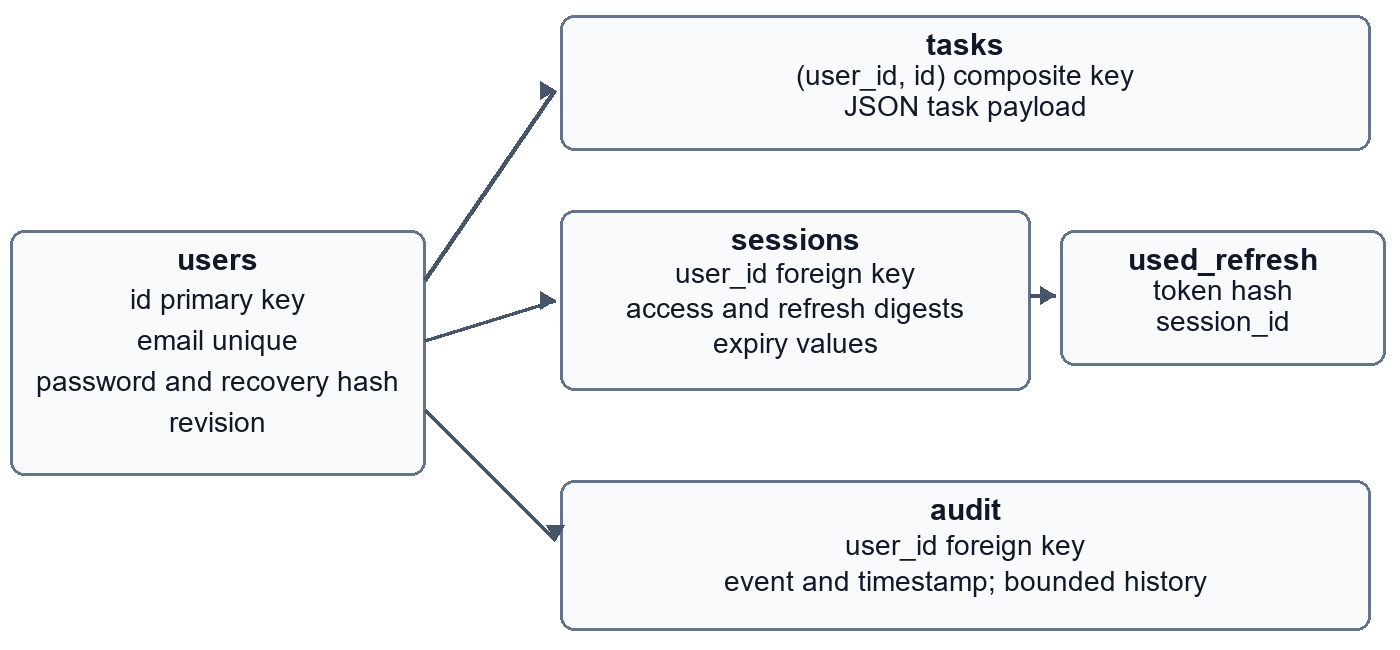
\includegraphics[width=\linewidth]{assets/data-model.png}\caption{SQLite ownership and session relationships}\end{figure}
Foreign-key deletion cascades keep dependent sessions, tasks and audit records associated with the owning account. A used refresh-token digest belongs to a session, allowing the service to recognize replay after token rotation. Password and token representations have different purposes: passwords use a salted password derivation function, while randomly generated session tokens are stored as digests. Neither mechanism means that the entire SQLite file is encrypted.

\section{Controller state and successful writes}
The controller exposes tasks, busy state and an error message. Before a mutation is allowed, a load must have succeeded. A failed reload invalidates that permission. Without this rule, an empty or stale in-memory collection could replace a saved snapshot whose contents were never successfully obtained. The guard is therefore a data-integrity requirement rather than simply a loading animation decision.

Mutation methods construct the proposed next collection and await repository persistence before publishing it as the controller's successful state. If saving fails, the previous collection remains authoritative in the UI, and an explicit retry or reload can be offered. Busy state prevents a second controller operation from overlapping the first. These decisions are covered at the controller and widget boundaries, but they do not by themselves guarantee that every editable form preserves later input.

\begin{figure}[htbp]\centering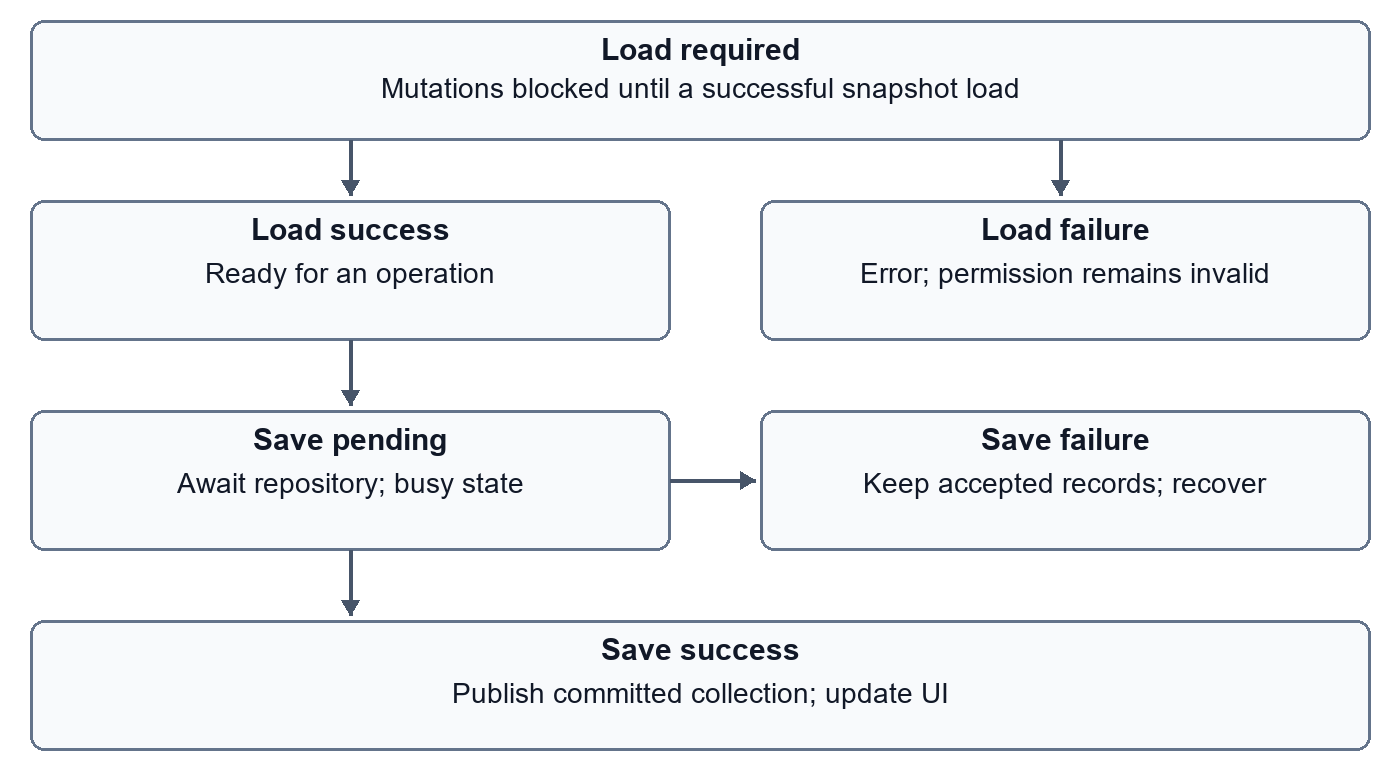
\includegraphics[width=\linewidth]{assets/state-flow.png}\caption{State transitions around loading and mutation}\end{figure}
Delete and undo follow the same persistence rule. The one-level session undo retains the deleted record and restores its complete data when valid. It is not a persistent recycle bin and does not promise recovery after closing the application. Tests compare the restored record, including metadata and identity, and verify that an unrelated record has not changed. Such assertions address accidental partial reconstruction more directly than a snackbar-only assertion.

\section{Remote concurrency and uncertain outcomes}
The HTTP repository loads both the task snapshot and its revision. A subsequent write supplies that revision. The server begins an immediate SQLite transaction, compares the expected revision, replaces only the owning user's collection, increments the revision and commits. A stale writer receives a conflict instead of overwriting changes based on an older snapshot. SQLite documents transactions and immediate transaction behavior; the account scoping and revision protocol are TaskFlow's own application design (SQLite, n.d.).

The client treats a failed remote write as an uncertain outcome. A connection failure can occur after the server commits but before the response reaches the client. Retrying the same assumed revision without reloading would be unsafe. The repository therefore invalidates its locally remembered revision after a write failure and requires a fresh load. This does not implement automatic conflict merging; it prioritizes avoiding an unexamined overwrite.

Whole-snapshot replacement is easy to reason about for the small test dataset and makes rollback assertions straightforward. Its cost is repeated transfer of records that did not change, and a broad conflict boundary when different clients edit different tasks. Per-task endpoints also exist on the server, but the inspected Flutter repository uses the snapshot route. A future change to per-record synchronization would require a new contract and tests for partial success, deletion conflicts and reconciliation rather than merely substituting an endpoint URL.

\section{Session security and operational limits}
The service uses random access and refresh tokens, stores their digests, rotates refresh tokens and can revoke sessions. Access lifetime is 15 minutes and session lifetime is seven days in the inspected configuration. A maximum of ten sessions per account bounds retained active sessions. Refresh-token reuse revokes the affected session family. Recovery codes are shown to the account owner and are not a substitute for email verification or an external identity provider.

The Flutter client keeps tokens in memory. Restarting the application therefore requires sign-in. A refresh request is shared when several requests need renewal, and generation checks stop an older asynchronous result from modifying a newer session. Wrong-current-password responses are distinguished from an expired authentication token. These are specific race and error-classification controls, not a claim of comprehensive security certification.

The backend uses salted scrypt hashes and bounded concurrent derivation work. Request size and request rates are bounded. Browser-origin restrictions do not replace server authorization. Non-loopback clients require HTTPS. These controls have not undergone an independent security assessment or sustained-load study.

\chapter{Implementation and platform behavior}
\section{Responsive workspace and interaction design}
The current interface uses a desktop-first workspace without removing the compact layout. A wide window places navigation beside the task canvas. The canvas groups progress, quick capture, search, discovery controls and task content. At smaller widths the layout adapts rather than retaining a desktop sidebar that would leave too little room for titles and form fields. Status and priority remain textually identifiable instead of being communicated by color alone.

The visual system uses a pale neutral application background, white surfaces, a restrained indigo accent and clear typographic hierarchy. Small shadows and borders separate surfaces without turning every control into a prominent card. The design goal is legibility and predictable action placement. This goal should not be confused with a measured rendering-performance improvement: the repository does not contain a frame-time study proving that the redesign eliminated jank.

\begin{figure}[htbp]\centering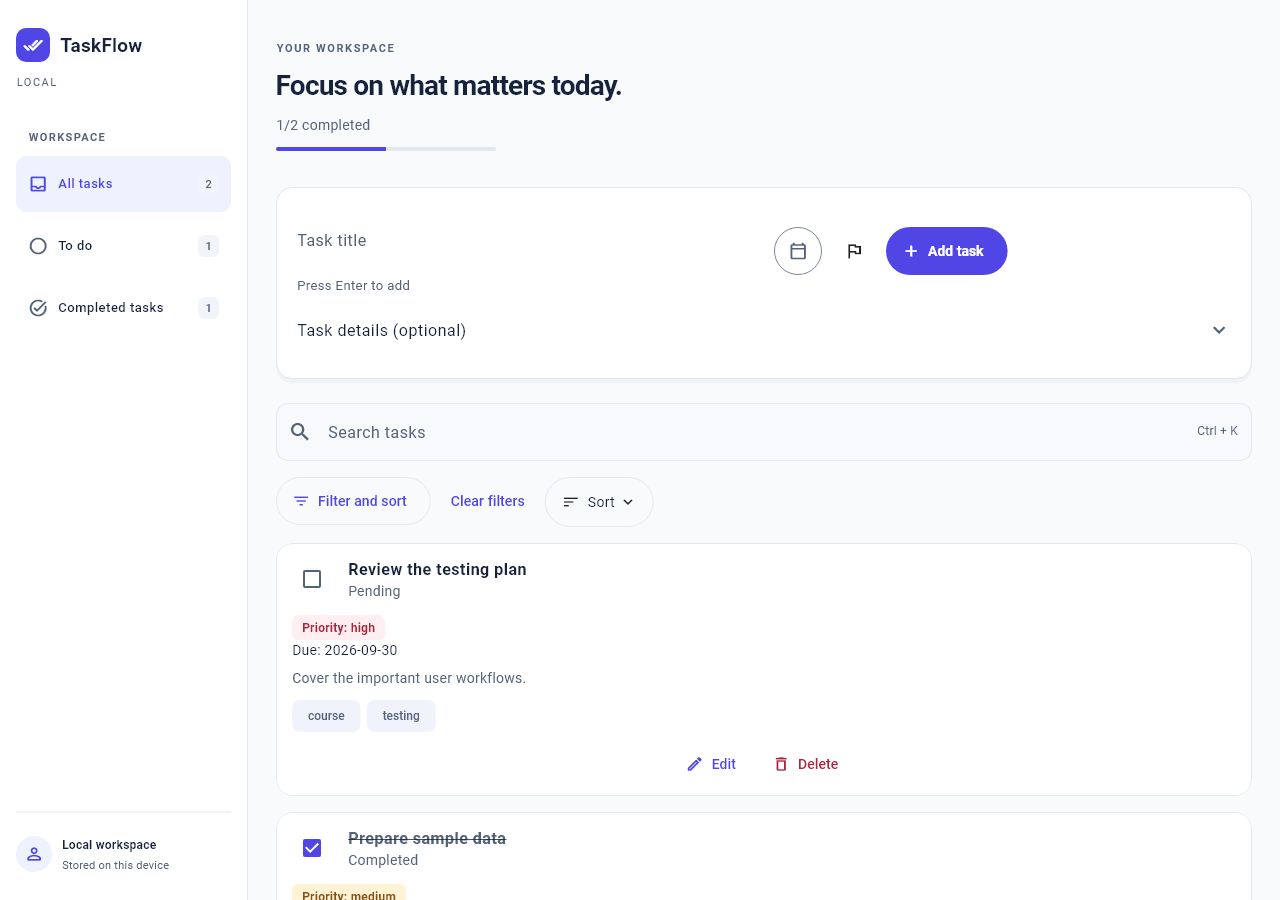
\includegraphics[width=\linewidth]{assets/ui-wide.png}\caption{Wide TaskFlow layout from the controlled golden fixture}\end{figure}
Figure 5.1 is a test-rendered fixture, not a photograph of a deployed production system. Its value is the inspectable arrangement and the maintained visual baseline. Runtime behavior requires the integration and browser evidence discussed later. The interface exposes a completion summary and navigation counts derived from task state, so a completion action has more than one observable effect that can be asserted.

\section{Capture and edit forms}
Quick capture accepts a title and optional task metadata. The Enter action provides a keyboard path in addition to the visible add control. Date and priority affordances keep frequent metadata close to capture, while additional details remain available. Required-field errors are shown in the form rather than only in a transient message. Validation tests check unsuccessful submission and correction, not just the presence of a validator function in source code.

The edit dialog retains a draft until a successful save. Dirty-state protection applies to explicit cancellation, Escape and back navigation, including raw date text that does not yet parse into a valid date. The pending-save state also constrains exit actions. Separate tests protect the distinction between a changed parsed value and invalid raw input; otherwise a user could type an invalid date and lose it because the form incorrectly considered itself unchanged.

Quick-create workspace exits likewise check whether a draft should be discarded. Each asynchronous save captures its submitted title and metadata. Completion resets the form only when its current draft still matches that submission; newer input is retained for the next task. Four controlled widget cases verify this behavior at compact and wide sizes for successful and unsuccessful writes, including duplicate-submit prevention and the subsequent save. These protections concern explicit workspace transitions. They do not establish a general operating-system-close, browser-refresh or crash-recovery guarantee.

\section{Discovery and stable results}
Search normalizes input and performs substring matching. The intentional-defect experiment deliberately violates that rule with prefix-only matching. Filters combine, so a result must satisfy the selected conditions rather than satisfying any single one. Sorting is stable and deterministic. Together these requirements enable exact list assertions: the test can compare the expected task set and order rather than accepting any nonempty result.

Search has a keyboard shortcut, and filter and sort controls retain meaningful labels. Clearing discovery conditions returns the user to an understandable state. A no-match result is distinct from an empty repository: the first invites changing the search or filters, while the second invites creating a task. Tests should preserve this distinction because showing the wrong empty state can hide a still-active filter and make a saved record appear lost.

\section{Loading and recoverable failures}
The loading state is not verified by waiting for an arbitrary delay and hoping the repository remains busy. A test-controlled completion gate holds the operation open. The test can then inspect disabled actions, the progress indication and draft state before releasing the operation. A separate failure path verifies the readable error and an explicit recovery action. This pattern makes intermediate UI states testable even when normal local storage is fast.

Save failures are tested independently from initial-load failures. They have different data risks: a failed initial load must not permit replacement of unknown data, while a failed save must preserve the previously accepted collection and useful draft input. Remote write failures also require revision recovery. A generic error screen alone would not establish these invariants, so the assertions inspect both visible state and repository results.

\section{Account workflows and backend integration}
The account gateway supports registration, sign-in and recovery. Signed-in settings expose profile, password, session and account-deletion actions. A task repository is scoped to the current account session. The application does not reuse a successful response from an older account generation to populate a later account's workspace. Backend tests exercise account isolation and concurrent writers, while the native online workflow crosses the actual HTTP and SQLite boundary.

The local server is started with the repository's PowerShell helper. The isolated online test uses synthetic accounts and a dedicated test database. Such accounts must not be created against a production service. The default loopback endpoint is suitable for the local development arrangement but is not a public deployment address. A physical Android device would require reachable networking and a suitable HTTPS backend for account-mode validation.

Node's SQLite module provides the database interface used by the server. The local runtime is Node 22.14.0; current online documentation may describe later versions, so runtime claims in this report are tied to the recorded environment rather than inferred from the newest documentation (Node.js, n.d.). No npm runtime dependency is required for the inspected backend. This reduces setup components but does not remove the need to monitor the runtime or assess deployment security.

\section{Platform and accessibility boundaries}
Windows supplies real native execution, local persistence and a release build in the retained evidence. Edge supplies real browser interactions, with an isolated harness for deterministic repository behavior and a separate account-lifecycle test. Historical hosted Android evidence supplies an emulator-based native gate and APK artifacts at an earlier revision. These forms of evidence complement each other; they cannot be combined into a claim that the newest interface has been manually tested on a physical Android phone.

Automated accessibility checks cover selected semantics, target-size and contrast conditions, form traversal and enlarged text. Flutter's accessibility testing documentation describes programmatic guidelines that assist such checks (Flutter, n.d.-g). The full manual screen-reader and page-wide keyboard protocol remains unexecuted in the retained status. A meaningful semantics tree is a necessary part of access, but it does not prove the quality of a complete spoken interaction.

Responsive tests also have a precise boundary. A logical viewport override verifies layout under that supplied size. It is not evidence of dragging a physical desktop window or using an Android input method. Native tests register and unregister the injected text-input channel to avoid Windows IME interference; consequently, those tests do not validate an actual IME. These limitations guide the next manual checks rather than invalidating the narrower automated evidence.

\chapter{Testing experiments and evaluation}
\section{Evaluation protocol and evidence identity}
Evaluation separates source identity, test selection, environment and observed outcome. The evaluated working tree is baseline 39dd199 plus the draft-consistency update. On 13 September 2026, the updated Flutter suite ran with coverage enabled, the Node API suite ran locally and the Windows draft-exit case passed. Logs are retained under \nolinkurl{docs/evidence/capture-fix/.} These fresh checks are distinct from the retained desktop UI milestone and earlier Android CI. No historical result is relabelled as a new execution.

The local Flutter environment is Flutter 3.47.1 with Dart 3.13.1 on Windows 11, build 26200.9445. The backend uses Node 22.14.0 and the runtime's built-in SQLite support. Android SDK availability differs between the local and earlier hosts. This report therefore uses the dated hosted Android record rather than implying that the present machine executed Android tests during preparation.

{\fontsize{11}{14}\selectfont\setlength{\tabcolsep}{4pt}\renewcommand{\arraystretch}{1.15}
\begin{longtable}{@{}>{\raggedright\arraybackslash}p{0.21\linewidth}>{\raggedright\arraybackslash}p{0.34\linewidth}>{\raggedright\arraybackslash}p{\dimexpr0.45\linewidth-16pt\relax}@{}}
\caption{Results and their actual verification boundaries}\\\toprule
\textbf{CHECK} & \textbf{RECORDED OUTCOME} & \textbf{BOUNDARY AND QUALIFICATION} \\ \midrule
\endfirsthead\toprule
\textbf{CHECK} & \textbf{RECORDED OUTCOME} & \textbf{BOUNDARY AND QUALIFICATION} \\ \midrule
\endhead
Flutter analysis & PASS during report preparation & Static analysis, not runtime correctness \\ \addlinespace[5pt]
Flutter suite with coverage & 100 cases PASS on 13 September & Includes four new draft-consistency cases; no coverage percentage asserted \\ \addlinespace[5pt]
Node API suite & 14 cases PASS on 13 September & Local HTTP, account and SQLite behaviors \\ \addlinespace[5pt]
Windows workflows & Draft-exit case PASS; historical 11-case selection PASS & New exit check distinguished from retained native/API workflows \\ \addlinespace[5pt]
Windows release build & PASS in retained minimal UI evidence & Build result, not a clean-machine install certificate \\ \addlinespace[5pt]
Edge UI harness & Final 1 of 1 run PASS after corrections & Four earlier failed attempts retained; not a five-run success result \\ \addlinespace[5pt]
Android hosted gate & 9 executions PASS at 9ca2a96 & Historical API 36 emulator evidence, not the newest UI revision \\ \addlinespace[5pt]
\bottomrule\end{longtable}}
The 100-case result is not added to 15 golden images as though they were unrelated test populations. Golden comparisons are included in the Flutter suite and maintain 15 unchanged baseline images. Similarly, the historical 11 native cases describe selected Windows workflows rather than 11 different platforms. Counting is useful for locating evidence, but the acceptance conditions determine what those counts mean.

\section{Scenario design and assertion strength}
The fresh-create scenario begins with isolated storage, observes an empty state, submits a valid record and checks its appearance. A validation scenario submits invalid input, observes readable validation, corrects the form and verifies a successful save. Discovery scenarios seed known records and assert normalized search, combined filters and exact ordering. Edit, completion, delete and undo scenarios compare full records and unaffected tasks where appropriate.

The persisted suite resets only its dedicated test preference keys. It does not clear all preferences on the host. A fresh repository and UI remount then verifies that persisted records can be read back. This is stronger than checking the previous widget's in-memory list, but it remains a remount rather than terminating and restarting the operating-system process. The distinction is stated because both actions are sometimes described imprecisely as a restart.

Independent controlled-repository cases exercise compact and wide validation, seeded discovery and recovery from load or write failures. Each case receives a fresh repository and resets its viewport. Completion gates make the pending interval observable. The online Windows scenario adds the actual API and isolated SQLite store. Separating these cases makes a failure easier to localize than a single long scenario that depends on the records created by every preceding step.

An adequate assertion checks the intended invariant. After editing, retaining the identifier and metadata matters. After filtering, exact membership matters. After deleting one task, preserving another matters. After retry, preventing duplicate writes matters. These are stronger oracles than merely checking that no exception escaped, or that a button responded to a tap.

\section{Intentional semantic defect}
The intentional-defect experiment asks whether UI automation detects a search error that leaves compilation and basic navigation intact. The correct implementation uses normalized substring matching. The temporary faulty patch replaces that comparison with prefix matching. The fixture contains Review Flutter testing and Write report, and the query includes surrounding whitespace and uppercase text: FLUTTER. The first task should still match because normalization and substring search are both required.

The baseline regression test passed before the change. With the faulty comparison, the expected task could not be found and the command failed. Restoring substring matching made the same regression pass again. The repository retains the buggy patch, corrected patch and unedited baseline, failure and recovery logs. The permanent test remains in the corrected source tree; the production implementation is not left intentionally defective.

{\fontsize{11}{14}\selectfont\setlength{\tabcolsep}{4pt}\renewcommand{\arraystretch}{1.15}
\begin{longtable}{@{}>{\raggedright\arraybackslash}p{0.21\linewidth}>{\raggedright\arraybackslash}p{0.34\linewidth}>{\raggedright\arraybackslash}p{\dimexpr0.45\linewidth-16pt\relax}@{}}
\caption{Deliberate search-defect experiment}\\\toprule
\textbf{STAGE} & \textbf{OBSERVATION} & \textbf{INTERPRETATION} \\ \midrule
\endfirsthead\toprule
\textbf{STAGE} & \textbf{OBSERVATION} & \textbf{INTERPRETATION} \\ \midrule
\endhead
Baseline & One regression case PASS, exit 0 & Correct search satisfies this fixture \\ \addlinespace[5pt]
Fault injection & Same case FAIL, exit 1 & Prefix-only search loses a middle-word match \\ \addlinespace[5pt]
Correction & Same case PASS, exit 0 & Restored substring behavior satisfies the oracle \\ \addlinespace[5pt]
\bottomrule\end{longtable}}
This experiment supports RQ2 with a genuine semantic failure rather than a fabricated log or a deliberately invalid syntax change. It does not estimate mutation score or general defect-detection probability. Only one selected defect and one regression case were used, with one recorded run at each stage. Broader mutation testing could be useful later, but it is not a result of this experiment.

\section{Test-level timing experiment}
A separate experiment recorded three rounds of selected test levels on one Windows host. Each command used a fresh Flutter invocation, with the order rotated across rounds and dependencies already resolved. The measured duration is whole-command wall time, including process startup and, for native execution, build and launch overhead. The selected workloads are unequal: four unit cases, one widget case, eight golden cases and four native controlled-repository cases.

{\fontsize{11}{14}\selectfont\setlength{\tabcolsep}{4pt}\renewcommand{\arraystretch}{1.15}
\begin{longtable}{@{}>{\raggedright\arraybackslash}p{0.21\linewidth}>{\raggedright\arraybackslash}p{0.34\linewidth}>{\raggedright\arraybackslash}p{\dimexpr0.45\linewidth-16pt\relax}@{}}
\caption{Whole-command duration in seconds for the selected suites}\\\toprule
\textbf{SELECTION} & \textbf{THREE RECORDED DURATIONS IN SECONDS} & \textbf{ARITHMETIC MEAN IN SECONDS} \\ \midrule
\endfirsthead\toprule
\textbf{SELECTION} & \textbf{THREE RECORDED DURATIONS IN SECONDS} & \textbf{ARITHMETIC MEAN IN SECONDS} \\ \midrule
\endhead
Unit, 4 cases & 4.707 / 4.360 / 5.499 & 4.855 \\ \addlinespace[5pt]
Widget, 1 case & 6.111 / 6.436 / 6.733 & 6.427 \\ \addlinespace[5pt]
Golden, 8 cases & 8.857 / 8.074 / 7.113 & 8.015 \\ \addlinespace[5pt]
Windows integration, 4 cases & 41.812 / 40.525 / 38.814 & 40.384 \\ \addlinespace[5pt]
\bottomrule\end{longtable}}
All twelve selected commands passed. Within this setup, the native selection required substantially more wall time than the other selected commands. That observation helps justify running narrow tests during development before the larger native gate. It does not establish a fair per-test speed ranking, because the scenario counts and assertions differ, nor does it predict cold-cache CI duration.

The small sample cannot support a general reliability estimate. Three successful repetitions can reveal an immediate deterministic failure, but rare timing failures may remain unseen. Warm caches and one host also restrict external validity. The most useful conclusion is procedural: retain raw results, state the workload and rotate order, then avoid converting a small local experiment into an unsupported universal comparison.

\section{Browser automation and maintenance findings}
The browser harness is compiled through an explicit QA entry point and uses synthetic in-memory data. It can hold repository operations and inject failures without touching account data or preferences. A separate real API scenario covers account task lifecycle. These two forms of browser testing must be reported independently because the controlled harness does not establish actual persistence or network behavior.

During the desktop redesign, the harness initially searched for an old heading. A later attempt assumed the input's accessible name was unchanged after focus, while the observed name included a second line. The corrected script checks the intended first line and verifies the active input before typing. Four failed attempts and the final successful run are retained. This is evidence of automation maintenance after a legitimate UI change, not evidence that four application defects were found and fixed.

The earlier browser stability experiment and multi-session work remain useful historical observations, but the current one-run success cannot inherit their repetition count. The script also retains raw outputs and exit codes and restores the default Web build after the harness. Those safeguards improve the reproducibility of evidence collection. They do not prove that all browsers, clean machines or assistive technologies behave identically.

\section{Threats to validity and remaining gates}
Internal validity depends on using independent fixtures and meaningful assertions. A fake may model an error more simply than a real transport failure, so a passing recovery test is not a complete network proof. Golden results depend on fonts and rendering environment. Test-level timings include overhead and unequal work. Browser-script corrections change the measurement procedure, which is why previous failed attempts remain visible rather than being replaced.

External validity is limited by the small coursework dataset, the selected Windows host and historical emulator configuration. The eager task list has not been stress-tested at the server's 500-record acceptance limit. No frame-time or sustained API-load study is reported. A successful APK build or hosted emulator test does not establish manual physical-device installation, account-mode connectivity on Android or production signing.

Construct validity also matters. Automated accessibility guidelines do not equal a complete screen-reader review, and successful remount does not equal process restart. Passing the selected checks does not imply absence of bugs. These distinctions prevent convenience metrics, especially total test count, from replacing the actual user risks under evaluation.

The next evidence gates are manual screen-reader and whole-page keyboard testing, clean-machine setup, release-artifact installation and current-revision Android verification where the environment allows it. Submission readiness additionally requires closure of open engineering findings, the team's presentation video and a confirmed contribution record. These items remain separate from the document's formatting and narrative completion.

\chapter{Conclusion}
\section{Findings}
TaskFlow answers RQ1 through risk-based test allocation. Unit tests isolate rules, widget tests expose interaction states, goldens protect reviewed visuals, and native or browser workflows cross additional runtime boundaries. No single level replaces the others.

For RQ2, the permanent search regression detected the temporary prefix-only defect and passed after correction. Retained patches and outputs support this narrow, reproducible result, not a general detection probability.

For RQ3, isolated fixtures, injected dependencies and completion gates make pending, failed and committed states inspectable. The study demonstrates their use without claiming a measured reduction in flakiness.

For RQ4, results remain tied to their platforms and revisions. The selected existing suites passed, but these results do not establish absence of defects.

\section{Prioritized continuation}
The project should complete its ongoing engineering review, execute the documented manual accessibility and clean-environment checks, and refresh platform evidence after relevant code changes. These actions address remaining evidence gaps without expanding the midterm into unrelated product features.

Final submission requires student verification and presentation materials. The demonstration should explain each workflow's assertions, execution boundary and remaining uncertainty, using the retained success and failure records.

\chapter*{References}\addcontentsline{toc}{chapter}{References}
\noindent\hangindent=0.75cm\hangafter=1 Flutter. (n.d.-a). Testing Flutter apps. Retrieved September 13, 2026, from \nolinkurl{https://docs.flutter.dev/testing/overview}\par\medskip
\noindent\hangindent=0.75cm\hangafter=1 Flutter. (n.d.-b). WidgetTester pump method. Retrieved September 13, 2026, from \nolinkurl{https://api.flutter.dev/flutter/flutter_test/WidgetTester/pump.html}\par\medskip
\noindent\hangindent=0.75cm\hangafter=1 Flutter. (n.d.-c). WidgetTester pumpAndSettle method. Retrieved September 13, 2026, from \nolinkurl{https://api.flutter.dev/flutter/flutter_test/WidgetTester/pumpAndSettle.html}\par\medskip
\noindent\hangindent=0.75cm\hangafter=1 Flutter. (n.d.-d). CommonFinders byKey method. Retrieved September 13, 2026, from \nolinkurl{https://api.flutter.dev/flutter/flutter_test/CommonFinders/byKey.html}\par\medskip
\noindent\hangindent=0.75cm\hangafter=1 Flutter. (n.d.-e). matchesGoldenFile function. Retrieved September 13, 2026, from \nolinkurl{https://api.flutter.dev/flutter/flutter_test/matchesGoldenFile.html}\par\medskip
\noindent\hangindent=0.75cm\hangafter=1 Flutter. (n.d.-f). Integration testing. Retrieved September 13, 2026, from \nolinkurl{https://docs.flutter.dev/testing/integration-tests}\par\medskip
\noindent\hangindent=0.75cm\hangafter=1 Flutter. (n.d.-g). Accessibility testing. Retrieved September 13, 2026, from \nolinkurl{https://docs.flutter.dev/ui/accessibility/accessibility-testing}\par\medskip
\noindent\hangindent=0.75cm\hangafter=1 LeanCode. (n.d.). Patrol documentation. Retrieved September 13, 2026, from \nolinkurl{https://patrol.leancode.co/documentation}\par\medskip
\noindent\hangindent=0.75cm\hangafter=1 Mai, V. M. (2024). Guidelines by Teacher Manh [Course report guidance supplied to the team].\par\medskip
\noindent\hangindent=0.75cm\hangafter=1 Microsoft. (n.d.). Locators. Playwright. Retrieved September 13, 2026, from \nolinkurl{https://playwright.dev/docs/locators}\par\medskip
\noindent\hangindent=0.75cm\hangafter=1 Node.js. (n.d.). SQLite. Retrieved September 13, 2026, from \nolinkurl{https://nodejs.org/api/sqlite.html}\par\medskip
\noindent\hangindent=0.75cm\hangafter=1 SQLite. (n.d.). Transaction. Retrieved September 13, 2026, from \nolinkurl{https://www.sqlite.org/lang_transaction.html}\par\medskip
\noindent\hangindent=0.75cm\hangafter=1 TaskFlow project. (2026). TaskFlow QA Lab [Source code and test evidence, revision 39dd199]. \nolinkurl{https://github.com/cross-platform-mobile-team/CROSS-PLATFORM-MOBILE-APP-DEVELOPMENT-Midterm-Project/tree/39dd199d9325f007fddf427622706d7de1419d38}\par\medskip
\noindent\hangindent=0.75cm\hangafter=1 Ton Duc Thang University. (2026). Cross-Platform Mobile App Development 503107 midterm assignment, semester 1, academic year 2026–2027 [Course brief, 503107-Essay-V2 (1).pdf, supplied to the team].\par\medskip
\noindent\hangindent=0.75cm\hangafter=1 Ton Duc Thang University. (2024). Template English and report guidelines [Faculty template and formatting materials supplied to the team].\par\medskip
\appendix
\chapter{Reproduction guide}
\section{Environment and safe setup}
Check out branch main-test and record the exact source revision before repeating a result. Use the pinned project SDK expectations and resolved pubspec.lock. On the report-preparation machine, Flutter is installed at \nolinkurl{C:/Users/LENOVO/flutter-sdk} and is not on PATH. Run flutter --version, dart --version, flutter doctor -v and flutter devices before selecting a native target. The commands below assume the corresponding executables are on PATH; otherwise use their full paths. Do not install an SDK or change system configuration merely to reproduce a document claim.

Run flutter pub get, then flutter analyze and flutter test --coverage. The backend gate is node --test backend/\nolinkurl{test/*.test.js.} Keep output and exit status together. The report does not publish a coverage percentage because a percentage was not calculated and checked for this manuscript. A generated coverage file alone should not be converted into an invented coverage claim.

Run native suites in separate invocations. The selected files are \nolinkurl{integration_test/independent_scenarios_test.dart,} \nolinkurl{integration_test/persisted_scenarios_test.dart,} \nolinkurl{integration_test/quick_create_exit_test.dart} and \nolinkurl{integration_test/windows_workflow_test.dart.} Use flutter test followed by the actual file and -d windows. Verify the current filenames against the repository before execution. The real API workflow is orchestrated by \nolinkurl{scripts/test-online-windows.ps1} with an isolated service and database. Never direct synthetic test accounts or destructive account tests at a production endpoint.

For browser reproduction, inspect \nolinkurl{scripts/test-edge-harness.ps1} and its supported parameters. It manages a QA build, server and isolated browser session, retains logs and restores the default Web build. The harness is a controlled in-memory test surface, not a replacement for the separate online browser lifecycle evidence. Output folders are unique and must not be overwritten to hide unsuccessful attempts.

\section{Deliberate defect safety}
The intentional-defect package is \nolinkurl{docs/evidence/intentional_defect.} Read its README before using either patch. Reproduce the defect only in an isolated worktree, run \nolinkurl{test/widget/search_regression_test.dart,} then restore the corrected implementation and rerun the same test. Do not leave the faulty search in the development branch. A patch failing to apply to a later revision requires inspection, not forceful replacement of unrelated work.

Additional engineering findings and their original diagnostics are maintained separately in \nolinkurl{docs/report/DEFERRED_REVIEW.md} for a later manuscript update. They are outside the selected experiment results reported here and have not been relabelled as passing checks.

\chapter{Evidence index}
{\fontsize{11}{14}\selectfont\setlength{\tabcolsep}{4pt}\renewcommand{\arraystretch}{1.15}
\begin{longtable}{@{}>{\raggedright\arraybackslash}p{0.21\linewidth}>{\raggedright\arraybackslash}p{0.34\linewidth}>{\raggedright\arraybackslash}p{\dimexpr0.45\linewidth-16pt\relax}@{}}
\caption{Evidence packages used in this report}\\\toprule
\textbf{PACKAGE OR FILE} & \textbf{PURPOSE} & \textbf{INTERPRETATION} \\ \midrule
\endfirsthead\toprule
\textbf{PACKAGE OR FILE} & \textbf{PURPOSE} & \textbf{INTERPRETATION} \\ \midrule
\endhead
\nolinkurl{docs/evidence/manifest.md} & Master evidence inventory & Consult dated sections and source revisions \\ \addlinespace[5pt]
\nolinkurl{docs/evidence/minimal-ui-20260913} & Current UI milestone logs & Windows, Flutter, API and corrected Edge run \\ \addlinespace[5pt]
\nolinkurl{docs/evidence/intentional_defect} & Baseline, faulty patch, fail log and fix pass & One selected search defect \\ \addlinespace[5pt]
\nolinkurl{docs/experiments/test-levels-20260909.md} & Experiment method and timing summary & Unequal workloads, three rounds, one host \\ \addlinespace[5pt]
\nolinkurl{docs/evidence/test-levels-20260909} & Raw timing outputs & Whole-command wall time \\ \addlinespace[5pt]
\nolinkurl{docs/evidence/android-ci-20260909.md} & Hosted Android result & Historical revision 9ca2a96 \\ \addlinespace[5pt]
\nolinkurl{docs/accessibility-testing.md} & Automated scope and manual protocol & Manual protocol remains unexecuted \\ \addlinespace[5pt]
\nolinkurl{docs/report/evidence} & Fresh report-preparation suite logs & Additional review tracked separately \\ \addlinespace[5pt]
\bottomrule\end{longtable}}
\chapter{Submission verification}
The recorded team is Nguyễn Bá Hùng, student ID 523K0006, and Nguyễn Bảo Long, student ID 523K0014. Both members belong to class 23K50201, Faculty of Information Technology, major Software Engineering. The instructor is Mai Văn Mạnh. Submission date, signatures and individual contribution allocation require confirmation by the team; no percentage or signed declaration is supplied here.

Before submission, both members should verify the report against the final source revision, reproduce the central workflows and explain the intentional defect. The final source package must retain configuration examples and dependencies but exclude secrets and generated caches. The course additionally requires a usable English presentation video within its time limit and meaningful participation by every member. Report completion does not substitute for those deliverables.

\end{document}